\documentclass[italian]{article}
\usepackage[T1]{fontenc}
\usepackage{graphicx}
\usepackage{mathtools}
\usepackage{amssymb}
\usepackage{amsthm}
\usepackage{xcolor}
\usepackage{nameref}
\usepackage{babel}
\usepackage[hidelinks]{hyperref}
\graphicspath{img/}
\title{Ingegneria dei requisiti}
\author{Riccardo Torre}
\begin{document}
	\maketitle
	\tableofcontents
	\section{Introduzione}
	Una soluzione software corretta viene applicata per risolvere alcuni dei problemi del mondo reale. È importante comprendere il \textbf{contesto} e i \textbf{problemi} del \textbf{mondo reale}.
	Viene riportato l'esempio del freno a mano di una macchina a guida autonoma.
	Il \textbf{problema} è rappresentato dal fatto che in certe situazioni potrebbe non essere conveniente togliere il freno a mano. Il \textbf{contesto} è rappresentato da molteplici situazioni, quali ad esempio: la macchina è in movimento, la macchina sta frenando, le intenzioni dell'autista, le regole di sicurezza, e così via\dots

	\paragraph{Terminologia: mondo e macchina.} Il \textbf{mondo} è usato come riferimento a tutte le problematiche del mondo reale. Può contenere \textbf{componenti umane}, come le organizzazioni, gli staff, gli operatori\dots, ma anche delle \textbf{componenti fisiche} come i dispositivi, il software legacy, i sensori, gli attuatori, madre natura (le componenti fisiche vanno modellate correttamente e fanno parte di madre natura)\dots
	Quando ci si utilizza il termine \textbf{macchina} si fa riferimento al mondo dei computer che sono dei contenitori software e hardware.

	L'ingegneria dei requisiti si occupa:
	\begin{itemize}
		\item dell'\textbf{effetto} che il software ha sul mondo reale;
		\item delle \textbf{proprietà} del mondo reale che il software deve tenere in considerazione.
	\end{itemize}
	\begin{figure}[th]
		\centering
		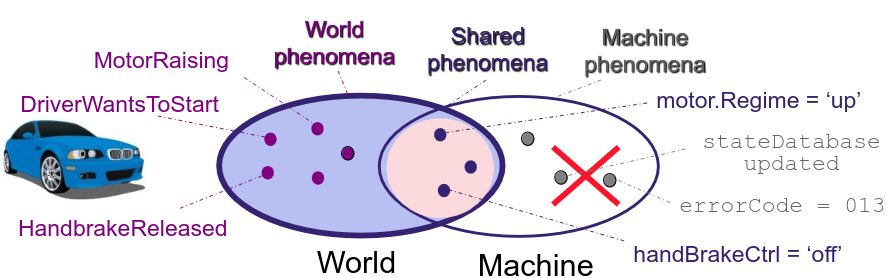
\includegraphics[width=0.7\linewidth]{img/word-machine-sets}
		\caption{modellazione dei problemi che sono contenuti nel mondo reale e delle soluzioni che sono contenute nella macchina.}
		\label{fig:word-machine-sets}
	\end{figure}
	Nella figura \ref{fig:word-machine-sets} vengono rappresentati, il \textbf{mondo reale}, e il \textbf{mondo delle macchine}, ovvero il software.

	Di seguito, viene indicato con $W$ il mondo reale e con $M$ il mondo delle macchine.
	\begin{itemize}
		\item $W \setminus M$: è la parte che rappresenta tutti i fenomeni del mondo reale che non interagiscono con il software. Ad esempio, l'accensione del motore, il rilascio del freno a mano, l'evento che l'utente vuole iniziare a guidare.
		\item $W \cap M$: appartengono tutti quei fenomeni che vengono modellati dal software. Ad esempio, il controllo del freno è spento, oppure il controllore del regime del motore è impostato ad "up".
		\item $M \setminus W$: sono i fenomeni che appartengono esclusivamente al mondo del software. Ad esempio, lo stato del database ad "aggiornato", oppure un codice di errore (errorCode = 013).
	\end{itemize}
	I requisiti descrivono l'informazione che appartiene solo all'insieme $W$, dunque sono legati esclusivamente al funzionamento del mondo reale e non ad aspetti che riguardano solamente il software.

	Esistono due versioni del mondo:
	\begin{enumerate}
		\item \textbf{System-as-is}: è la descrizione del mondo, prima dell'introduzione del sistema software.
		\item \textbf{System-to-be}: è la descrizione del mondo nel quale il sistema opera.
	\end{enumerate}
	\begin{figure}[th]
		\centering
		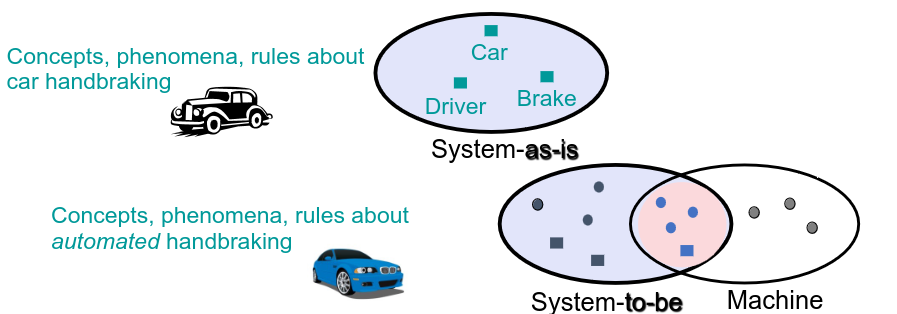
\includegraphics[width=0.7\linewidth]{img/system-as-is-system-to-be}
		\caption{system-as-is e system-to-be.}
		\label{fig:system-as-is-system-to-be}
	\end{figure}
	In generale l'\textbf{ingegneria dei requisiti} si occupa di coordinare un insieme di attività che ci permettono di esplorare, valutare, documentare, consolidare, revisionare ed adattare gli obbiettivi, le funzionalità, le qualità, i vincoli e le assunzioni di un software.
	I \textbf{requisiti di sistema} fanno parte del system-to-be. I \textbf{requisiti del software} fanno parte del software-to-be e sono le funzionalità che deve fornire per rispondere ai requisiti richiesti dall'utente.
	\begin{figure}[th]
		\centering
		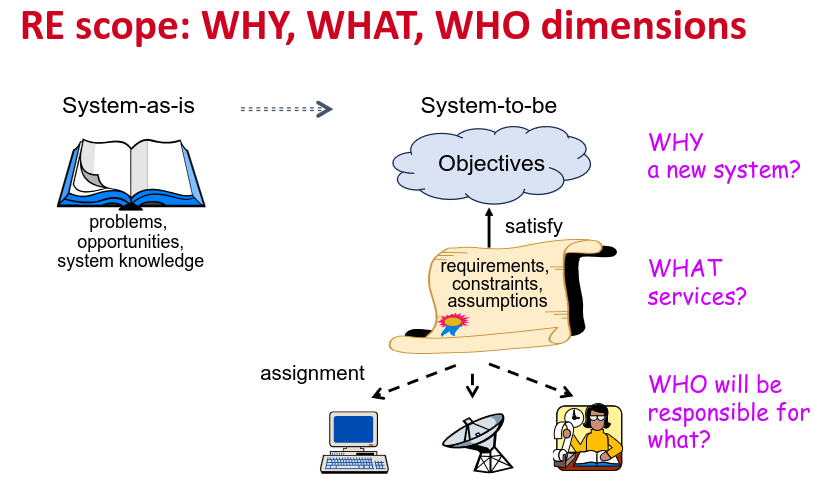
\includegraphics[width=0.7\linewidth]{img/www-dimensions}
		\caption{il chi, che cosa e perché dell'ingegneria dei requisiti.}
		\label{fig:www-dimensions}
	\end{figure}

	Per comprendere appieno il system-to-be (figura \ref{fig:www-dimensions}) bisogna comprendere quali sono gli \emph{obbiettivi} del sistema (\textbf{perché} è necessario un nuovo sistema), bisogna stabilire quali \emph{servizi e funzionalità} sono necessari per soddisfare gli obbiettivi del sistema, descrivendo i vincoli, le assunzioni e i requisiti (\textbf{che cosa}). Deve essere chiaro anche \textbf{chi} ha la \emph{responsabilità} di fornire i servizi (componenti software, dispositivi fisici oppure operatori umani) e quali sono i \emph{ruoli}.

	I registri per descrivere i requisiti possono essere:
	\begin{itemize}
		\item \textbf{descrittivo:} si concentra sulla definizione di proprietà, indipendentemente dalle funzionalità del sistema. Potrebbero dipendere dalle leggi naturali, dai vincoli fisici, e così via. Ad esempio, un requisito descrittivo potrebbe essere:
		\begin{quotation}
			\textit{"Se le porte del treno sono chiuse, allora non sono aperte."}
		\end{quotation}
		Oppure:
		\begin{quotation}
			\textit{"Se l'accelerazione del treno è positiva, allora la sua velocità è non nulla."}
		\end{quotation}
		\item \textbf{prescrittiva:} proprietà desiderabili del sistema che potrebbero dipendere da come il sistema funziona.
		\begin{quotation}
			\textit{Le porte dovrebbero sempre rimanere chiuse quando il treno è in movimento}
		\end{quotation}
	\end{itemize}
	\paragraph{\textbf{Nota bene!}}I vincoli prescrittivi possono essere negoziati tra gli ingegneri dei requisiti e i vari stakeholders, possono essere indeboliti o rimpiazzati con alternative, mentre i vincoli descrittivi no.

	I requisiti possono riferirsi a fenomeni dell'\textbf{ambiente} (ad esempio, se il treno si sta muovendo, le porte devono essere chiuse) oppure possono essere condivisi tra il software-to-be e l'ambiente (una componente software potrebbe monitorare un fenomeno ambientale e avvisare un'altra componente software del cambiamento avvenuto. Ad esempio, se la velocità monitorata è pari a zero, allora lo stato delle porte deve essere chiuso).

	Un \textbf{requisito di sistema} ha delle frasi tipicamente \textbf{prescrittive} che si riferiscono ai fenomeni ambientali e che devono essere formulate con vocabolario che deve essere comprensibile a tutti gli stakeholders. Ad esempio:
	\begin{quotation}
		\textit{Se il sistema è in movimento, allora le porte devono essere chiuse}
	\end{quotation}
	ovvero: $\text{TrainMoving} \implies \text{DoorsClosed}$.
	Un \textbf{requisito del software} contiene tipicamente delle frasi \textbf{prescrittive} che si riferiscono a fenomeni condivisi e che devono essere supportate dal software-to-be. Vengono formulate con un vocabolario comprensibile agli sviluppatori software. Un esempio è il seguente.
	\begin{quotation}
		\textit{"Se la velocità misurata è diversa da zero, allora le porte devono essere nello stato chiuso"}
	\end{quotation}
	ossia: $\text{measuredSpeed}\ne 0 \implies doorsState = \text{`closed'}$
	Tipi di frasi che possiamo formulare nei nostri domini possono essere:
	\begin{itemize}
		\item \textbf{Proprietà di dominio:} è una frase descrittiva riguardo un fenomeno del mondo reale che avviene indipendentemente dall'esistenza di un sistema software.
		Ad esempio: $\text{trainAcceleration} > 0 \implies \text{trainSpeed} \ne 0$
		\item \textbf{Assunzioni:} sono delle frasi che devono essere soddisfatte dall'ambiente quando deve essere considerato il software-to-be e formulate in riferimento a fenomeni ambientali. Generalmente sono prescrittive. Ad esempio
		$\text{measuredSpeed} \ne 0 \iff \text{trainSpeed} \ne 0$.
		\item \textbf{Definizioni:} sono frasi che forniscono un significato preciso al sistema. Non hanno un valore di verità. Ad esempio, una definizione potrebbe essere:
		\begin{quotation}
			\textit{measuredSpeed (velocità misurata) è la velocità stimata dal tachimetro del treno}.
		\end{quotation}
	\end{itemize}
	\begin{figure}[th]
		\centering
		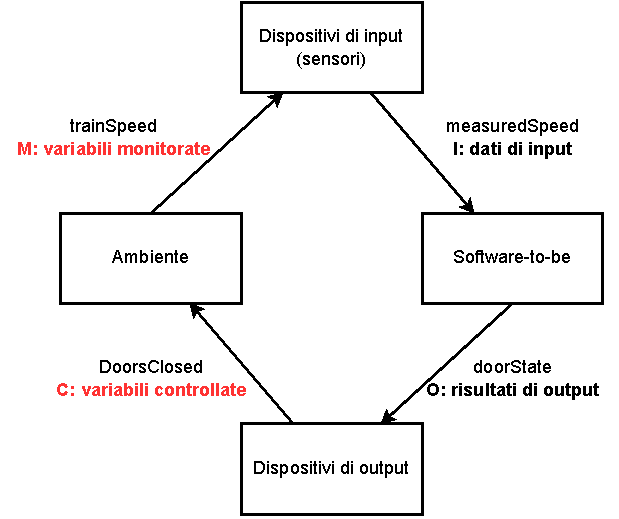
\includegraphics[width=0.7\linewidth]{img/modello-4-variabili.drawio}
		\caption{modello 4-variable.}
		\label{fig:modello-4-variabili}
	\end{figure}
	Il modello in figura \ref{fig:modello-4-variabili} è composto da:
	\begin{itemize}
		\item \textbf{dispositivi di input} quali ad esempio sensori;
		\item \textbf{softwareToBe} ovvero il software da sviluppare;
		\item \textbf{ambiente} nel quale il sistema opera;
		\item \textbf{dispositivi di output} ad esempio attuatori.
	\end{itemize}
	Il sistema misura la velocità attraverso i sensori. Il software in esecuzione nel sistema, legge i dati di input, prende delle decisioni, calcola dei risultati che successivamente invia agli attuatori. Gli attuatori rilevano i risultati e attuano delle azioni sul mondo esterno. In questa fase possono modificare delle variabili di controllo del mondo esterno (come quelle delle porte). Il mondo contiene sia le variabili controllate dagli attuatori, sia quelle monitorate dai dispositivi di input. Ad esempio la variabile che contiene l'informazione relativa alla velocità del treno, viene monitorata da uno o più sensori. Quindi la variabile monitorata è la velocità del treno, mentre la variabile controllata è le porte chiuse.
	\begin{itemize}
		\item 	$SysReq \subseteq M \times C$: i requisiti di sistema sono una relazione tra variabili monitorate e le variabili controllate. Le variabili controllate cambiano a seconda delle variabili monitorate;
		\item $SofReq \subseteq I \times O$: i requisiti software sono la relazione tra dati di input ed output;
		\item $SofReq = Map(SysReq, Dom, Asm)$: i requisiti software sono una mappa tra i requisiti di sistema ($SysReq$), le assunzioni ($Asm$) e le proprietà di dominio ($Dom$).
	\end{itemize}


\end{document}